\chapter{La vitesse des réactions}\label{ch:g12:reaction-rates}

Une bouteille de lait oubliée sur le plan de travail de la cuisine
tourne en un ou deux jours~; au réfrigérateur, elle se conserve plus
d'une semaine. Un feu d'artifice \omterm{def:g4:what-a-fire-needs:burning}{brûle} en une fraction de seconde, alors
qu'une statue en calcaire, dans un parc de la ville, s'altère au fil des
siècles. Les \omterm{def:g8:balanced-equations:equation}{équations ajustées} et les tableaux d'\omterm{def:g10:reaction-progress-table:extent}{avancement} disent ce
que donne une réaction, et en quelle quantité~; ils ne disent rien de sa
rapidité. Ce chapitre mesure la vitesse des réactions, cherche ce qui la
contrôle, et décrit la façon la plus simple dont une réaction peut
ralentir au fil de son \omterm{def:g10:reaction-progress-table:extent}{avancement}.

\begin{recall}
La concentration d'une solution (\cref{ch:g10:concentration-and-dilution})
et l'\omterm{def:g10:reaction-progress-table:extent}{avancement} d'une réaction (\cref{ch:g10:reaction-progress-table}).
L'\omterm{def:g11:absorbance:absorbance}{absorbance} d'une solution diluée est proportionnelle à la
concentration de l'espèce colorée (\cref{ch:g11:absorbance}). Un \omterm{def:g11:titration:titration}{titrage}
mesure la quantité d'une espèce (\cref{ch:g11:titration}).
\end{recall}

\begin{omfigure}
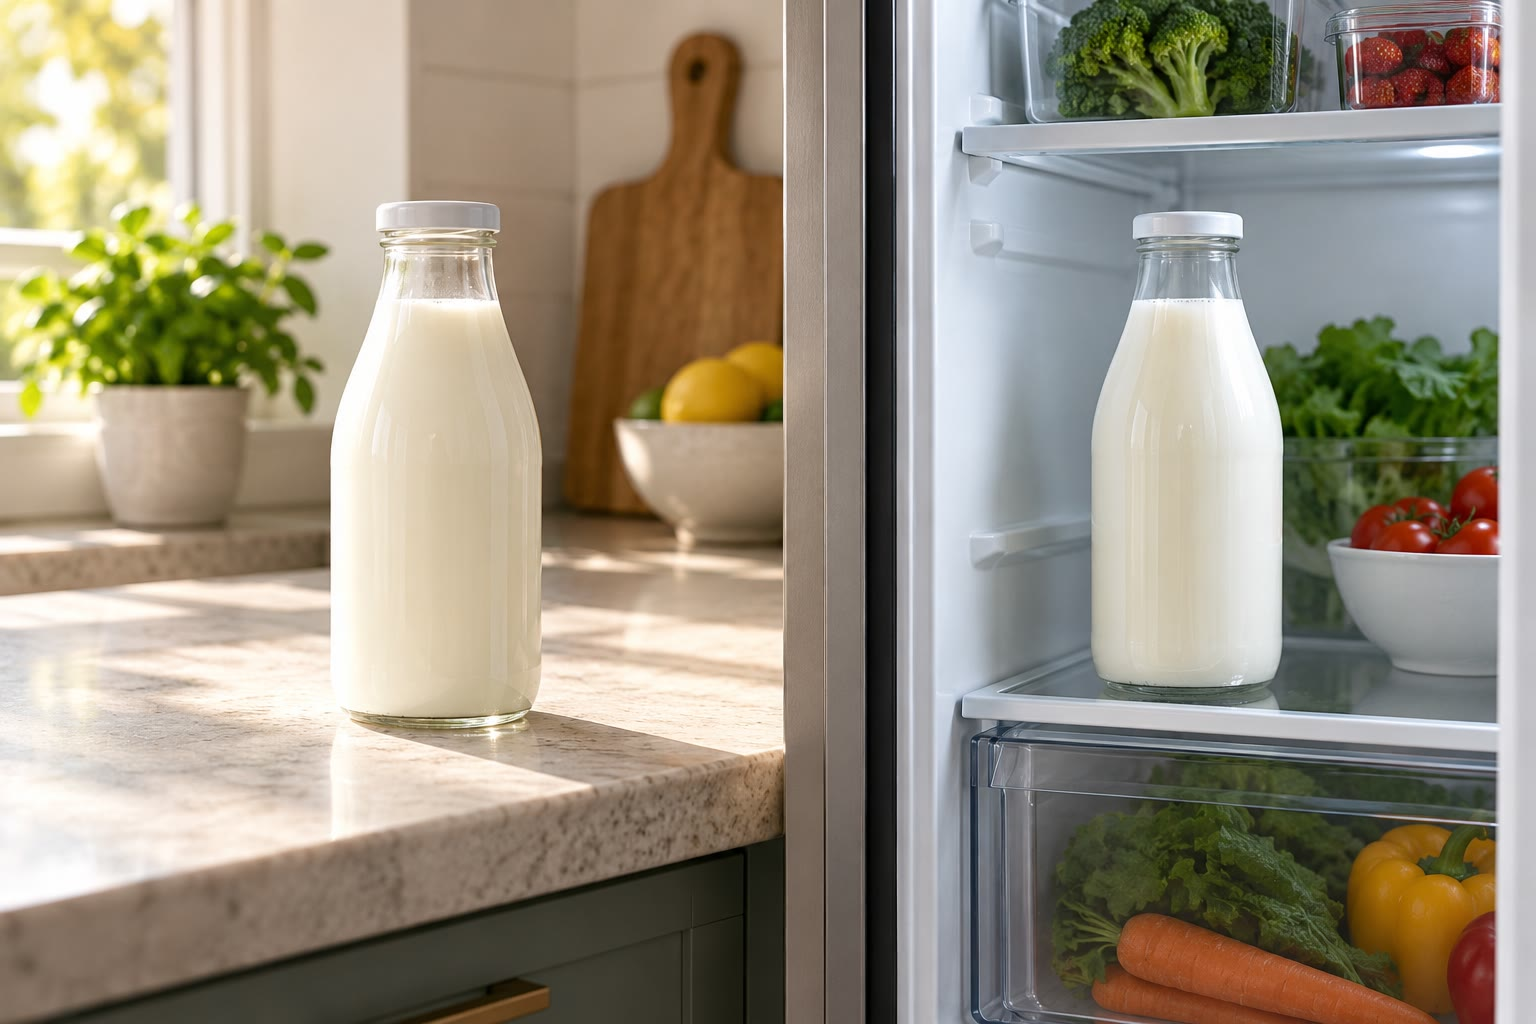
\includegraphics[width=0.48\linewidth]{images/book1/ai/g12-milk-counter-fridge.jpg}

{\small Le même lait, sur le plan de travail et au réfrigérateur~: les
réactions qui le font tourner sont plus lentes au froid.}
\end{omfigure}

\section{Suivre une réaction au cours du temps}

Certaines réactions sont terminées dès que les \omterm{def:g7:chemical-reactions:reactant}{réactifs} se rencontrent~:
la \omterm{def:g9:ions:precipitate}{précipitation} du chlorure d'argent, la réaction d'un acide avec une
base. D'autres durent des minutes, des heures ou des années. Pour
étudier une réaction lente, les chimistes mesurent la concentration d'un
\omterm{def:g7:chemical-reactions:reactant}{réactif} ou d'un produit à intervalles réguliers. Ils peuvent
\begin{itemize}
  \item prélever de petits échantillons, arrêter la réaction dans chacun
        d'eux, et les titrer~;
  \item mesurer l'\omterm{def:g11:absorbance:absorbance}{absorbance} de la solution, quand un \omterm{def:g7:chemical-reactions:reactant}{réactif} ou un
        produit est coloré~;
  \item mesurer la pression ou le volume d'un gaz dégagé, ou la
        conductivité d'une solution dont les \omterm{def:g9:ions:ion}{ions} changent.
\end{itemize}

\begin{definition}[Trempe]\label{def:g12:reaction-rates:quenching}
Effectuer la \emph{trempe}\index{trempe} d'un échantillon, c'est arrêter,
ou ralentir très fortement, la réaction qui s'y déroule au moment du
prélèvement, en général en le refroidissant brusquement et en le
diluant, de sorte que l'on puisse mesurer sa composition à loisir.
\end{definition}

\begin{inthelab}[Tremper un échantillon]
Toutes les cinq minutes, on prélève \qty{10.0}{mL} du \omterm{def:g6:pure-substances-and-mixtures:mixture}{mélange}
réactionnel à la pipette et on les verse dans un bécher contenant
environ \qty{40}{mL} d'eau glacée. Diluée cinq fois et refroidie vers
\qty{0}{\celsius}, la réaction devient si lente qu'on peut la considérer
comme arrêtée~; on titre alors l'échantillon. La date de l'échantillon
est l'instant où il a été versé dans l'eau glacée, et non celui du
\omterm{def:g11:titration:titration}{titrage}.
\end{inthelab}

\begin{omfigure}
\begin{tikzpicture}[font=\small, scale=0.8]
  \pic[transform shape] at (0,0) {erlenmeyer={0.4}{orange!25}};
  \node[anchor=north, align=center] at (0,-0.15) {mélange\\ réactionnel};
  \pic[transform shape, rotate=-35] at (1.4,1.2) {pipette={0.6}{orange!25}};
  \draw[omProp, very thick, -{Stealth}] (1.6,0.8) -- (2.9,0.8);
  \node[anchor=south] at (2.25,0.85) {\qty{10.0}{mL}};
  \pic[transform shape] at (4,0) {beaker={0.55}{cyan!12}};
  \foreach \p in {(3.6,0.4),(4.2,0.6),(3.9,0.85),(4.4,0.3)}
    \draw[black!30, fill=white] \p ++(-0.1,-0.08) rectangle ++(0.2,0.16);
  \node[anchor=north, align=center] at (4,-0.15) {eau glacée~:\\ réaction arrêtée};
  \draw[omProp, very thick, -{Stealth}] (5.1,0.8) -- (6.4,0.8);
  \pic[transform shape] at (7.5,0) {erlenmeyer={0.35}{orange!12}};
  \pic[transform shape] at (7.5,2.75) {burette={0.7}{violet!45}};
  \node[anchor=north, align=center] at (7.5,-0.15) {titrage de\\ l'échantillon};
\end{tikzpicture}

{\small Suivre une réaction par prélèvements~: prélever un échantillon,
le tremper, puis le doser à loisir.}
\end{omfigure}

\section{Les facteurs cinétiques}

\begin{definition}[Facteur cinétique]\label{def:g12:reaction-rates:kinetic-factor}
Un \emph{facteur cinétique}\index{facteur cinetique@facteur cinétique} est une grandeur
qui modifie la vitesse d'une réaction sans changer ce que donne la
réaction~: la température, les concentrations des \omterm{def:g7:chemical-reactions:reactant}{réactifs}, la surface
de contact entre \omterm{def:g7:chemical-reactions:reactant}{réactifs} de phases différentes, et la présence d'un
catalyseur (chapitre suivant).
\end{definition}

\begin{proposition}[Plus chaud, plus concentré, plus divisé~: plus rapide]\label{prop:g12:reaction-rates:factors}
En général, une réaction est plus rapide quand la température est plus
élevée, quand les \omterm{def:g7:chemical-reactions:reactant}{réactifs} sont plus concentrés et, pour un \omterm{def:g7:chemical-reactions:reactant}{réactif}
solide, quand il est plus finement divisé.
\end{proposition}

\begin{proof}
Admis, avec une image~: les particules qui réagissent doivent se
rencontrer, et se rencontrer assez violemment. Les concentrer rend les
rencontres plus fréquentes~; diviser un solide offre plus de surface de
rencontre~; chauffer les fait se déplacer plus vite, si bien qu'elles se
rencontrent plus souvent et, surtout, qu'une plus grande part des
rencontres est assez énergique pour rompre des liaisons.
\end{proof}

\begin{example}[Trois cas de la vie courante]\label{ex:g12:reaction-rates:everyday}
Les aliments se conservent plus longtemps au réfrigérateur, et bien plus
longtemps au congélateur~: les réactions qui les altèrent ralentissent
au froid. La fine poussière de farine en suspension dans l'\omterm{def:g4:air-a-mixture-of-gases:air}{air} d'un
moulin peut exploser, alors qu'un sac de farine ne fait que se consumer
lentement~: même réaction, surface de contact énorme. Un comprimé
effervescent \omterm{def:g2:mixing-and-dissolving:dissolve}{se dissout} plus vite dans l'eau si on l'écrase d'abord.
\end{example}

\begin{omfigure}
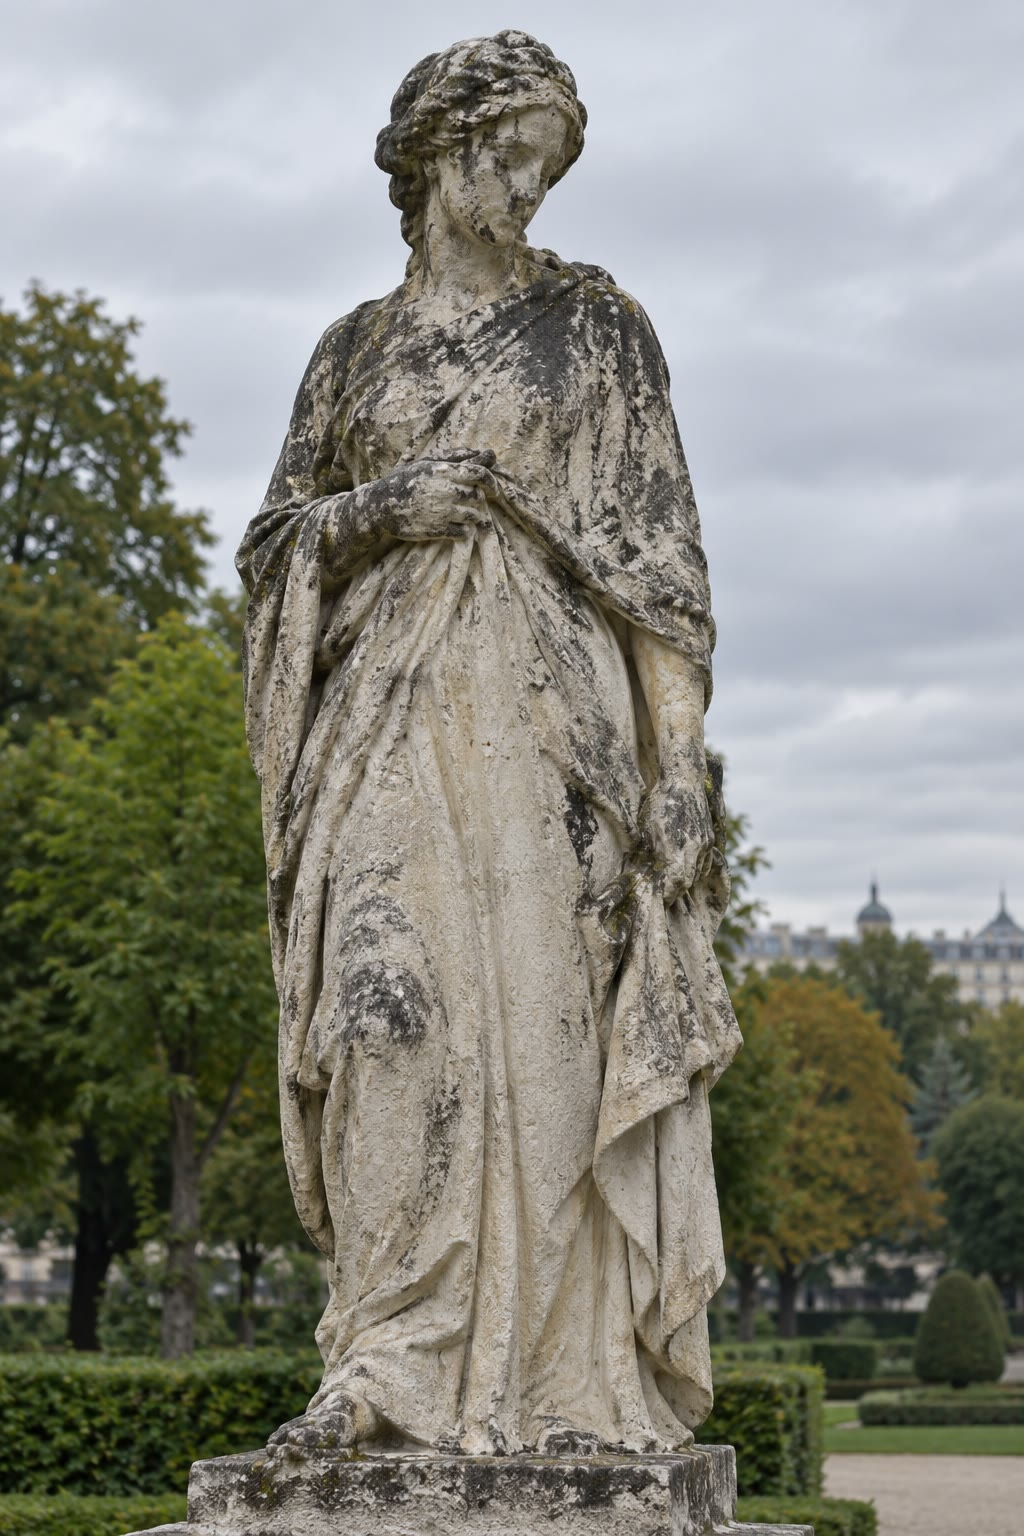
\includegraphics[width=0.42\linewidth,height=6cm,keepaspectratio]{images/book1/ai/g12-weathered-statue.jpg}

{\small Une statue en calcaire altérée par la pluie~: une réaction qui
dure des siècles.}
\end{omfigure}

\section{Vitesses de disparition et d'apparition}

\begin{definition}[Vitesse de disparition, vitesse d'apparition]\label{def:g12:reaction-rates:rate}
Dans une solution de volume constant, la \emph{vitesse de
disparition}\index{vitesse de disparition}
d'un \omterm{def:g7:chemical-reactions:reactant}{réactif} A à l'instant $t$ est
\[
  v_A(t) = -\frac{d[\ce{A}]}{dt},
\]
et la \emph{vitesse d'apparition}\index{vitesse d'apparition} d'un
produit P est $v_P(t) = \dfrac{d[\ce{P}]}{dt}$. Toutes deux sont
positives, en
\si{mol.L^{-1}.min^{-1}} (ou par seconde).
\end{definition}


\begin{method}[Lire une vitesse sur une tangente]\label{met:g12:reaction-rates:tangent}
\begin{enumerate}
  \item Sur la courbe de $[\ce{A}]$ en fonction de $t$, tracer la
        tangente à l'instant choisi.
  \item Lire deux points éloignés sur la tangente et calculer sa pente,
        $\Delta[\ce{A}] / \Delta t$.
  \item La \omterm{def:g12:reaction-rates:rate}{vitesse de disparition} est l'opposé de cette pente (pour un
        produit, la pente elle-même).
\end{enumerate}
\end{method}

\begin{omfigure}
\begin{tikzpicture}
\begin{axis}[width=0.8\linewidth, height=6.4cm, xmin=0, xmax=60, ymin=0,
    ymax=11, xlabel={$t$ (\si{min})}, ylabel={$[\ce{A}]$ (\si{mmol/L})},
    axis lines*=left, ymajorgrids, xmajorgrids, grid style={gray!20},
    tick label style={font=\small}, label style={font=\small},
    legend style={font=\small, at={(0.98,0.97)}, anchor=north east,
    draw=none, fill=white}, legend cell align=left]
  \addplot[very thick, omDef] table[x=t, y=A1] {figdata/out/grade-12-reaction-rates-a.dat};
  \addplot[very thick, omThm] table[x=t, y=A2] {figdata/out/grade-12-reaction-rates-a.dat};
  \addplot[thick, dashed, omProp, restrict y to domain=0:11] table[x=t, y=tangent]
    {figdata/out/grade-12-reaction-rates-a.dat};
  \legend{$k = \qty{0.050}{min^{-1}}$, $k = \qty{0.100}{min^{-1}}$ (plus chaud),
    tangente en $t = 0$}
  \addplot[densely dotted, black!60] coordinates {(0,5) (13.86,5) (13.86,0)};
  \addplot[densely dotted, black!60] coordinates {(6.93,5) (6.93,0)};
  \node[font=\small, anchor=south west] at (axis cs:14.6,5.4) {$t_{1/2} = \qty{13.9}{min}$};
  \node[font=\small, anchor=south east] at (axis cs:6.7,0.2) {\qty{6.9}{min}};
\end{axis}
\end{tikzpicture}

{\small La concentration d'un \omterm{def:g7:chemical-reactions:reactant}{réactif} A en fonction du temps, pour une
même \omterm{def:g12:reaction-rates:first-order}{réaction d'ordre 1} à deux températures. La tangente en $t = 0$ (en
tirets) donne la vitesse initiale~; les pointillés repèrent les \omterm{def:g12:reaction-rates:half-life}{temps de
demi-réaction}.}
\end{omfigure}

\begin{example}[La vitesse initiale]\label{ex:g12:reaction-rates:initial}
Sur la courbe bleue, la tangente en $t = 0$ va de \qty{10.0}{mmol/L} à
$t = 0$ à $0$ à $t = \qty{20}{min}$~: sa pente vaut
$-10.0/20 = \qty{-0.50}{mmol.L^{-1}.min^{-1}}$, donc la vitesse initiale
de disparition vaut \qty{0.50}{mmol.L^{-1}.min^{-1}}. Ensuite, la courbe
s'aplatit et la vitesse diminue~: la réaction ralentit à mesure que A
est consommé.
\end{example}

\section{Les réactions d'ordre 1}

\begin{definition}[Réaction d'ordre 1, constante de vitesse]\label{def:g12:reaction-rates:first-order}
Une réaction est une \emph{réaction d'ordre 1}\index{reaction d'ordre 1@réaction d'ordre 1}
par rapport à A si sa \omterm{def:g12:reaction-rates:rate}{vitesse de disparition} est proportionnelle, à
chaque instant, à la concentration de A~:
\[
  -\frac{d[\ce{A}]}{dt} = k\,[\ce{A}] .
\]
La constante positive $k$, en \si{min^{-1}} ou en \si{s^{-1}}, est la
\emph{constante de vitesse}\index{constante de vitesse}~; elle dépend de
la température.
\end{definition}

\begin{proposition}[Décroissance exponentielle]\label{prop:g12:reaction-rates:exponential}
Pour une \omterm{def:g12:reaction-rates:first-order}{réaction d'ordre 1} de concentration initiale $[\ce{A}]_0$,
\[
  [\ce{A}](t) = [\ce{A}]_0\, e^{-kt} .
\]
\end{proposition}

\begin{proof}
La fonction $f(t) = [\ce{A}]_0 e^{-kt}$ a pour dérivée
$f'(t) = -k [\ce{A}]_0 e^{-kt} = -k f(t)$~: elle vérifie donc l'équation
de vitesse, et $f(0) = [\ce{A}]_0$. Qu'elle soit la seule fonction de ce
type est admis ici (cela se démontre en mathématiques, pour les
équations $y' = ay$).
\end{proof}

\begin{method}[Tester l'ordre 1]\label{met:g12:reaction-rates:test}
\begin{enumerate}
  \item À partir des mesures, calculer $\ln [\ce{A}]$ (ou $\ln A$ pour
        une \omterm{def:g11:absorbance:absorbance}{absorbance} proportionnelle à $[\ce{A}]$) à chaque instant.
  \item Tracer $\ln[\ce{A}]$ en fonction de $t$~: comme
        $\ln[\ce{A}] = \ln[\ce{A}]_0 - kt$, les points sont alignés si et
        seulement si la réaction est d'ordre 1.
  \item La pente de la droite vaut $-k$.
\end{enumerate}
\end{method}

\section{Le temps de demi-réaction}

\begin{definition}[Temps de demi-réaction]\label{def:g12:reaction-rates:half-life}
Le \emph{temps de demi-réaction}\index{temps de demi-reaction@temps de demi-réaction} $t_{1/2}$
d'une réaction est la durée nécessaire pour que la concentration du
\omterm{def:g10:reaction-progress-table:limiting}{réactif limitant} atteigne la moitié de sa valeur initiale.
\end{definition}

\begin{proposition}[Temps de demi-réaction d'une réaction d'ordre 1]\label{prop:g12:reaction-rates:half-life}
Pour une \omterm{def:g12:reaction-rates:first-order}{réaction d'ordre 1},
\[
  t_{1/2} = \frac{\ln 2}{k},
\]
quelle que soit la concentration initiale~; au bout de $n$ \omterm{def:g12:reaction-rates:half-life}{temps de
demi-réaction}, la concentration est divisée par $2^n$.
\end{proposition}

\begin{proof}
$[\ce{A}]_0 e^{-k t_{1/2}} = [\ce{A}]_0 / 2$ donne $e^{-k t_{1/2}} = 1/2$,
donc $k t_{1/2} = \ln 2$. Chaque nouveau \omterm{def:g12:reaction-rates:half-life}{temps de demi-réaction}
multiplie de nouveau la concentration par $e^{-k t_{1/2}} = 1/2$.
\end{proof}


\begin{example}[Lire les temps de demi-réaction]\label{ex:g12:reaction-rates:half-lives}
Pour $k = \qty{0.050}{min^{-1}}$, $t_{1/2} = 0.693 / 0.050 =
\qty{13.9}{min}$~: la concentration passe de 10.0 à 5.0, puis 2.5, puis
\qty{1.25}{mmol/L} à 13.9, 27.7 et \qty{41.6}{min}. L'expérience plus
chaude, avec un $k$ deux fois plus grand, a un \omterm{def:g12:reaction-rates:half-life}{temps de demi-réaction}
deux fois plus court, \qty{6.9}{min}, comme le montre la figure.
\end{example}

\begin{remark}[Demi-vies en physique]\label{rem:g12:reaction-rates:radioactive}
En physique, on parle de demi-vie pour les noyaux radioactifs, dont le
nombre décroît de la même façon exponentielle~: une désintégration
radioactive se comporte comme une \omterm{def:g12:reaction-rates:first-order}{réaction d'ordre 1}. Le livre de
physique en traite.
\end{remark}

\begin{omfigure}
\begin{minipage}{0.49\linewidth}
\begin{tikzpicture}
\begin{axis}[width=\linewidth, height=5.4cm, xmin=0, xmax=26, ymin=0,
    ymax=0.85, xlabel={$t$ (\si{min})}, ylabel={absorbance $A$},
    axis lines*=left, ymajorgrids, grid style={gray!20},
    tick label style={font=\scriptsize}, label style={font=\small}]
  \addplot[only marks, mark=*, mark size=1.8pt, omDef] table[x=t, y=A]
    {figdata/out/grade-12-reaction-rates-b.dat};
  \addplot[thick, omProp, domain=0:26, samples=60] {0.8*exp(-0.11552*x)};
\end{axis}
\end{tikzpicture}
\end{minipage}\hfill
\begin{minipage}{0.49\linewidth}
\begin{tikzpicture}
\begin{axis}[width=\linewidth, height=5.4cm, xmin=0, xmax=26, ymin=-3.4,
    ymax=0, xlabel={$t$ (\si{min})}, ylabel={$\ln A$}, axis lines*=left,
    ymajorgrids, grid style={gray!20}, tick label style={font=\scriptsize},
    label style={font=\small}]
  \addplot[only marks, mark=*, mark size=1.8pt, omDef] table[x=t, y=lnA]
    {figdata/out/grade-12-reaction-rates-b.dat};
  \addplot[thick, omProp, domain=0:26] {-0.2231-0.11552*x};
\end{axis}
\end{tikzpicture}
\end{minipage}

{\small La décoloration du cristal violet en milieu basique (données du
problème du week-end). À gauche~: l'\omterm{def:g11:absorbance:absorbance}{absorbance} décroît selon une
exponentielle. À droite~: $\ln A$ en fonction de $t$ est une droite de
pente
$-\qty{0.116}{min^{-1}}$~: la réaction est d'ordre 1 par rapport au
colorant.}
\end{omfigure}

\section{Exercices}

\begin{exercise}[$\star$]\label{exo:g12:reaction-rates:1}
Nommer le \omterm{def:g12:reaction-rates:kinetic-factor}{facteur cinétique} en jeu dans chaque cas~: un réfrigérateur
conserve les aliments~; le sucre en poudre \omterm{def:g2:mixing-and-dissolving:dissolve}{se dissout} plus vite qu'un
morceau~; un acide plus concentré attaque le zinc plus vite~; une pomme
coupée brunit plus vite en été.
\end{exercise}

\begin{exercise}[$\star$]\label{exo:g12:reaction-rates:2}
Lire, sur la figure de $[\ce{A}]$ en fonction du temps, le \omterm{def:g12:reaction-rates:half-life}{temps de
demi-réaction} de chaque expérience.
Que vaut $[\ce{A}]$ sur la courbe bleue au bout de deux \omterm{def:g12:reaction-rates:half-life}{temps de
demi-réaction}~?
\end{exercise}

\begin{exercise}[$\star$]\label{exo:g12:reaction-rates:3}
La tangente à la courbe d'un produit, tracée en $t = \qty{5}{min}$,
passe par
$(0, \qty{1.0}{mmol/L})$ et $(\qty{10}{min}, \qty{5.0}{mmol/L})$.
Quelle est la \omterm{def:g12:reaction-rates:rate}{vitesse d'apparition} du produit à \qty{5}{min}~?
\end{exercise}

\begin{exercise}[$\star$]\label{exo:g12:reaction-rates:4}
Pourquoi verse-t-on un échantillon dans de l'eau glacée avant de le
titrer~? Pourquoi faut-il noter la date de l'échantillon au moment où
on le verse, et non au moment où on le titre~?
\end{exercise}

\begin{exercise}[$\star$]\label{exo:g12:reaction-rates:5}
Une \omterm{def:g12:reaction-rates:first-order}{réaction d'ordre 1} a un \omterm{def:g12:reaction-rates:half-life}{temps de demi-réaction} de \qty{10}{min}.
Quelle fraction du \omterm{def:g7:chemical-reactions:reactant}{réactif} reste-t-il au bout de \qty{30}{min}~? Au bout
de \qty{1}{h}~?
\end{exercise}

\begin{exercise}[$\star\star$]\label{exo:g12:reaction-rates:6}
Concentrations d'un \omterm{def:g7:chemical-reactions:reactant}{réactif}, en \si{mmol/L}~: 8.00 à \qty{0}{min}, 5.66
à \qty{5}{min}, 4.00 à \qty{10}{min}, 2.83 à \qty{15}{min}, 2.00 à
\qty{20}{min}. Calculer $\ln[\ce{A}]$ à chaque instant et montrer que la
réaction est d'ordre 1. Trouver $k$ et le \omterm{def:g12:reaction-rates:half-life}{temps de demi-réaction}.
\end{exercise}

\begin{exercise}[$\star\star$]\label{exo:g12:reaction-rates:7}
Une \omterm{def:g12:reaction-rates:first-order}{réaction d'ordre 1} a pour \omterm{def:g12:reaction-rates:half-life}{temps de demi-réaction}
$t_{1/2} = \qty{25}{s}$. Calculer $k$.
\end{exercise}

\begin{exercise}[$\star\star$]\label{exo:g12:reaction-rates:8}
Pour $[\ce{A}]_0 = \qty{0.100}{mol/L}$ et $k = \qty{0.020}{min^{-1}}$,
calculer $[\ce{A}]$ au bout de 10, 30 et \qty{100}{min}.
\end{exercise}

\begin{exercise}[$\star\star$]\label{exo:g12:reaction-rates:9}
Sur la figure de $[\ce{A}]$ en fonction du temps, estimer la pente de la
courbe bleue en $t = \qty{13.9}{min}$ (tracer une tangente), et la
comparer à
$-k[\ce{A}]$ à cet instant.
\end{exercise}

\begin{exercise}[$\star\star$]\label{exo:g12:reaction-rates:10}
Le diiode \ce{I2}, brun, se forme lentement dans une solution incolore.
L'\omterm{def:g11:absorbance:absorbance}{absorbance} augmente de 0 vers 0.60. Expliquer pourquoi l'\omterm{def:g11:absorbance:absorbance}{absorbance}
permet de suivre $[\ce{I2}]$, et comment on lit la \omterm{def:g12:reaction-rates:rate}{vitesse d'apparition}
à un instant donné sur la courbe de $A$ en fonction de $t$.
\end{exercise}

\begin{exercise}[$\star\star$]\label{exo:g12:reaction-rates:11}
Deux expériences de la même réaction partent de $[\ce{A}]_0 = 10$ et
\qty{20}{mmol/L}. Si la réaction est d'ordre 1, comparer leurs vitesses
initiales et leurs \omterm{def:g12:reaction-rates:half-life}{temps de demi-réaction}.
\end{exercise}

\begin{exercise}[$\star\star\star$]\label{exo:g12:reaction-rates:12}
Combien de \omterm{def:g12:reaction-rates:half-life}{temps de demi-réaction} faut-il à une \omterm{def:g12:reaction-rates:first-order}{réaction d'ordre 1} pour
qu'il ne reste que \qty{1}{\percent} de son \omterm{def:g7:chemical-reactions:reactant}{réactif}~?
\qty{0.1}{\percent}~? Donner la formule générale de la durée nécessaire
pour descendre à une fraction $f$.
\end{exercise}

\begin{exercise}[$\star\star\star$]\label{exo:g12:reaction-rates:13}
Une réaction a pour constante $k = \qty{0.050}{min^{-1}}$ à
\qty{20}{\celsius} et
$k = \qty{0.100}{min^{-1}}$ à \qty{30}{\celsius}. Combien de temps
faut-il pour consommer \qty{90}{\percent} du \omterm{def:g7:chemical-reactions:reactant}{réactif} à chaque
température~? Une règle empirique courante dit que la vitesse double
tous les \qty{10}{\celsius}~: cette réaction la suit-elle~?
\end{exercise}

\begin{exercise}[$\star\star\star$]\label{exo:g12:reaction-rates:14}
On \omterm{def:g12:reaction-rates:quenching}{trempe} un échantillon en versant \qty{5.0}{mL} dans \qty{45}{mL}
d'eau glacée. Donner deux raisons pour lesquelles la réaction devient
beaucoup plus lente. Si la réaction est d'ordre 1 par rapport à chacun
de deux \omterm{def:g7:chemical-reactions:reactant}{réactifs}, par quel facteur la seule \omterm{def:g10:concentration-and-dilution:dilution}{dilution} divise-t-elle la
vitesse~?
\end{exercise}

\begin{exercise}[$\star\star\star$]\label{exo:g12:reaction-rates:15}
Montrer, en dérivant, que la \omterm{def:g12:reaction-rates:rate}{vitesse de disparition} d'une \omterm{def:g12:reaction-rates:first-order}{réaction
d'ordre 1} est elle-même une fonction exponentielle du temps,
$v(t) = k[\ce{A}]_0 e^{-kt}$. Quelle est la vitesse initiale~? Au bout de
combien de temps la vitesse vaut-elle la moitié de la vitesse
initiale~?
\end{exercise}

\section{Problème~: le colorant qui pâlit}

\begin{problem}[{Problème du week-end --- le cristal violet décoloré par
les ions hydroxyde~: combien de temps avant que la couleur ait presque
disparu~?}]
\label{pb:g12:reaction-rates:1}
Le cristal violet, un colorant violet, réagit avec les \omterm{def:g9:ions:ion}{ions} hydroxyde en
donnant un produit incolore. En large excès d'\omterm{def:g9:ions:ion}{ions} hydroxyde, la vitesse
ne dépend que de la concentration du colorant. On enregistre
l'\omterm{def:g11:absorbance:absorbance}{absorbance} de la solution à la longueur d'onde où le colorant absorbe
le plus~:
\begin{center}
\small
\begin{tabular}{l*{10}{c}}
\hline
$t$ (\si{min}) & 0 & 2 & 4 & 6 & 8 & 10 & 12 & 15 & 20 & 25 \\
$A$ & 0.800 & 0.639 & 0.501 & 0.402 & 0.315 & 0.255 & 0.199 & 0.143 &
0.078 & 0.046 \\
\hline
\end{tabular}
\end{center}

\medskip
\noindent\textbf{Partie I --- \omterm{def:g11:absorbance:absorbance}{Absorbance} et concentration.}
\begin{enumerate}
  \item Pourquoi l'\omterm{def:g11:absorbance:absorbance}{absorbance} est-elle proportionnelle à la
        concentration du colorant~? Quelle condition la solution doit-elle
        remplir~?
  \item Pourquoi le produit, incolore, n'est-il pas vu à cette longueur
        d'onde~?
  \item Pourquoi utilise-t-on les \omterm{def:g9:ions:ion}{ions} hydroxyde en large excès~?
  \item Que lirait-on sur le spectrophotomètre en fin de réaction~?
\end{enumerate}

\medskip
\noindent\textbf{Partie II --- La réaction est-elle d'ordre 1~?}
\begin{enumerate}[resume]
  \item Lire directement le \omterm{def:g12:reaction-rates:half-life}{temps de demi-réaction} dans le tableau.
  \item Vérifier qu'il est le même de $t = 6$ à $t = 12$ min.
  \item Calculer $\ln A$ pour chaque instant.
  \item Tracer $\ln A$ en fonction de $t$ (ou utiliser la figure du
        chapitre). Qu'observe-t-on~? Conclure.
  \item Calculer la pente à partir des points à 0 et à \qty{20}{min}.
\end{enumerate}

\medskip
\noindent\textbf{Partie III --- La \omterm{def:g12:reaction-rates:first-order}{constante de vitesse}.}
\begin{enumerate}[resume]
  \item En déduire $k$.
  \item Calculer le \omterm{def:g12:reaction-rates:half-life}{temps de demi-réaction} à partir de $k$, et le
        comparer à celui de la question 5.
  \item Calculer la vitesse initiale de disparition du colorant,
        exprimée comme une vitesse de diminution de l'\omterm{def:g11:absorbance:absorbance}{absorbance}.
  \item Quel serait le \omterm{def:g12:reaction-rates:half-life}{temps de demi-réaction} si l'\omterm{def:g11:absorbance:absorbance}{absorbance} initiale
        valait 0.400~?
\end{enumerate}

\medskip
\noindent\textbf{Partie IV --- Prévision.}
\begin{enumerate}[resume]
  \item Prévoir l'\omterm{def:g11:absorbance:absorbance}{absorbance} à \qty{30}{min}.
  \item À quel instant l'\omterm{def:g11:absorbance:absorbance}{absorbance} descend-elle à 0.008, soit
        \qty{1}{\percent} de sa valeur de départ~?
  \item Combien de \omterm{def:g12:reaction-rates:half-life}{temps de demi-réaction} cela représente-t-il~?
  \item L'œil ne voit plus la couleur au-dessous de $A = 0.010$
        environ. Quand la solution paraît-elle incolore~?
  \item On recommence l'expérience à une température plus élevée de
        \qty{10}{\celsius}, et le \omterm{def:g12:reaction-rates:half-life}{temps de demi-réaction} devient
        \qty{3.0}{min}. Quand atteint-on \qty{1}{\percent}~?
  \item Donner la réponse finale~: combien de \omterm{def:g12:reaction-rates:half-life}{temps de demi-réaction} la
        couleur met-elle pour descendre à \qty{1}{\percent} de sa valeur
        de départ, et combien de minutes cela fait-il ici~?
\end{enumerate}
\end{problem}
